% !TEX encoding = UTF-8 Unicode
% !TEX program = pdflatex
% !TEX spellcheck = en_US


% In order to correctly compile this document,
% execute the following commands:
% 1. pdflatex
% 2. pdflatex
% 3. pdflatex



\documentclass[amsthm,ebook]{saparticle}

% IF YOU USE PDFLATEX
\usepackage[utf8x]{inputenc}
% if you write in english and in greek
\usepackage{ucs}
\usepackage[greek,english]{babel}
\languageattribute{greek}{polutoniko}

% IF YOU USE XELATEX
%\usepackage{polyglossia}
% if you write in italian
%\setmainlanguage{italian}
% If you want put some ancient greek:
%\setotherlanguage[variant=polytonic]{greek}
%\newfontfamily{\greekfont}[Ligatures=TeX]{Palatino Linotype}

% dummy text (remove in a normal thesis)
% remove if not necessary
\usepackage{siunitx}
%Natbib for bibliography management
\usepackage[authoryear]{natbib}
% custom commands
\newcommand{\bs}{\textbackslash}

%%%%%%%%
%TITLE:%
%%%%%%%%
\title{EDB 2.0.
How EAGLE improved the Epigraphic Database Bari}
\author[uniba]{Anita Rocco \corref{first}}
\address[uniba]{Dip. di Studi Umanistici, Università degli Studi di Bari ``Aldo Moro''}
\cortext[first]{Corresponding author. Email: anita.rocco@uniba.it}
\begin{document}
\maketitle
\begin{abstract}
This paper is dedicated to the evolution of the Epigraphic Database Bari (EDB) from the minimalistic design of its
origins to its current status. Although EDB, the database of inscriptions by Christians from Rome, dates back to the
late 1980s , involvement in the EAGLE – Europeana project has had a significantly positive impact on its development.
In fact, maintaining its peculiar character, dictated by its own history and, mostly, by the characteristics of its
documentary base, it has taken advantage of the solutions adopted to integrate different archives and purpose-built
best practices. 
\end{abstract}
\keywords{Epigraphic database, EDB, EAGLE Europeana, Christian inscriptions, Late antique inscriptions }










\section{Introduction}


\noindent The Epigraphic Database Bari (EDB) is an `old' database, it dates back to the late 1980s , when Carlo Carletti\footnote{
He was professor of \emph{Epigrafia e antichità cristiane} in the former \emph{Department of Classical and Christian Studies} of Bari
University.}, inspired by Jory's experience indexing CIL VI\footnote{\citet{_corpus_1974}. The six volumes of the
computerized KeyWord-In-Context index to all the approximately 40,000 texts collected in the sixth volume of the \emph{Corpus
Inscriptionum Latinarum} (CIL) are the outcome of a trailblazing work of arrangement and organization of the
inscriptions in a \emph{database}, even if limited to their textual part.}, started a project of digitization of the
inscriptions commissioned by Christians from Rome between the third and eighth centuries, collected and edited in the
27,688 lemmas of the ICVR\footnote{\emph{The Corpus of Inscriptiones christianae urbis Romae} started in 1922 by A. Silvagni,
was published, mostly, by A. Ferrua, later supported by D. Mazzoleni and C. Carletti, between 1956 and 1992. Pursuing
the work of G.B. de Rossi of the mid-1800s (IC), ICVR registers the inscriptions by Christians found in the suburban
area of Rome, sorted in topographic order by consular road, then by catacomb. Inscriptions found inside the urban walls
or the recently discovered suburban ones aren’t yet included in the ICVR volumes.}. The data were stored in a data
processing program, called ICVR, running under MS-DOS, later converted to a database for Microsoft Access. It was
originally intended for internal use only.

Since its very beginnings the database has been designed on the basis of a conceptual model, which conveys the
complexity of epigraphs even in the frame of a very simple and basic IT structure.



\begin{figure}[hbp]
\centering
 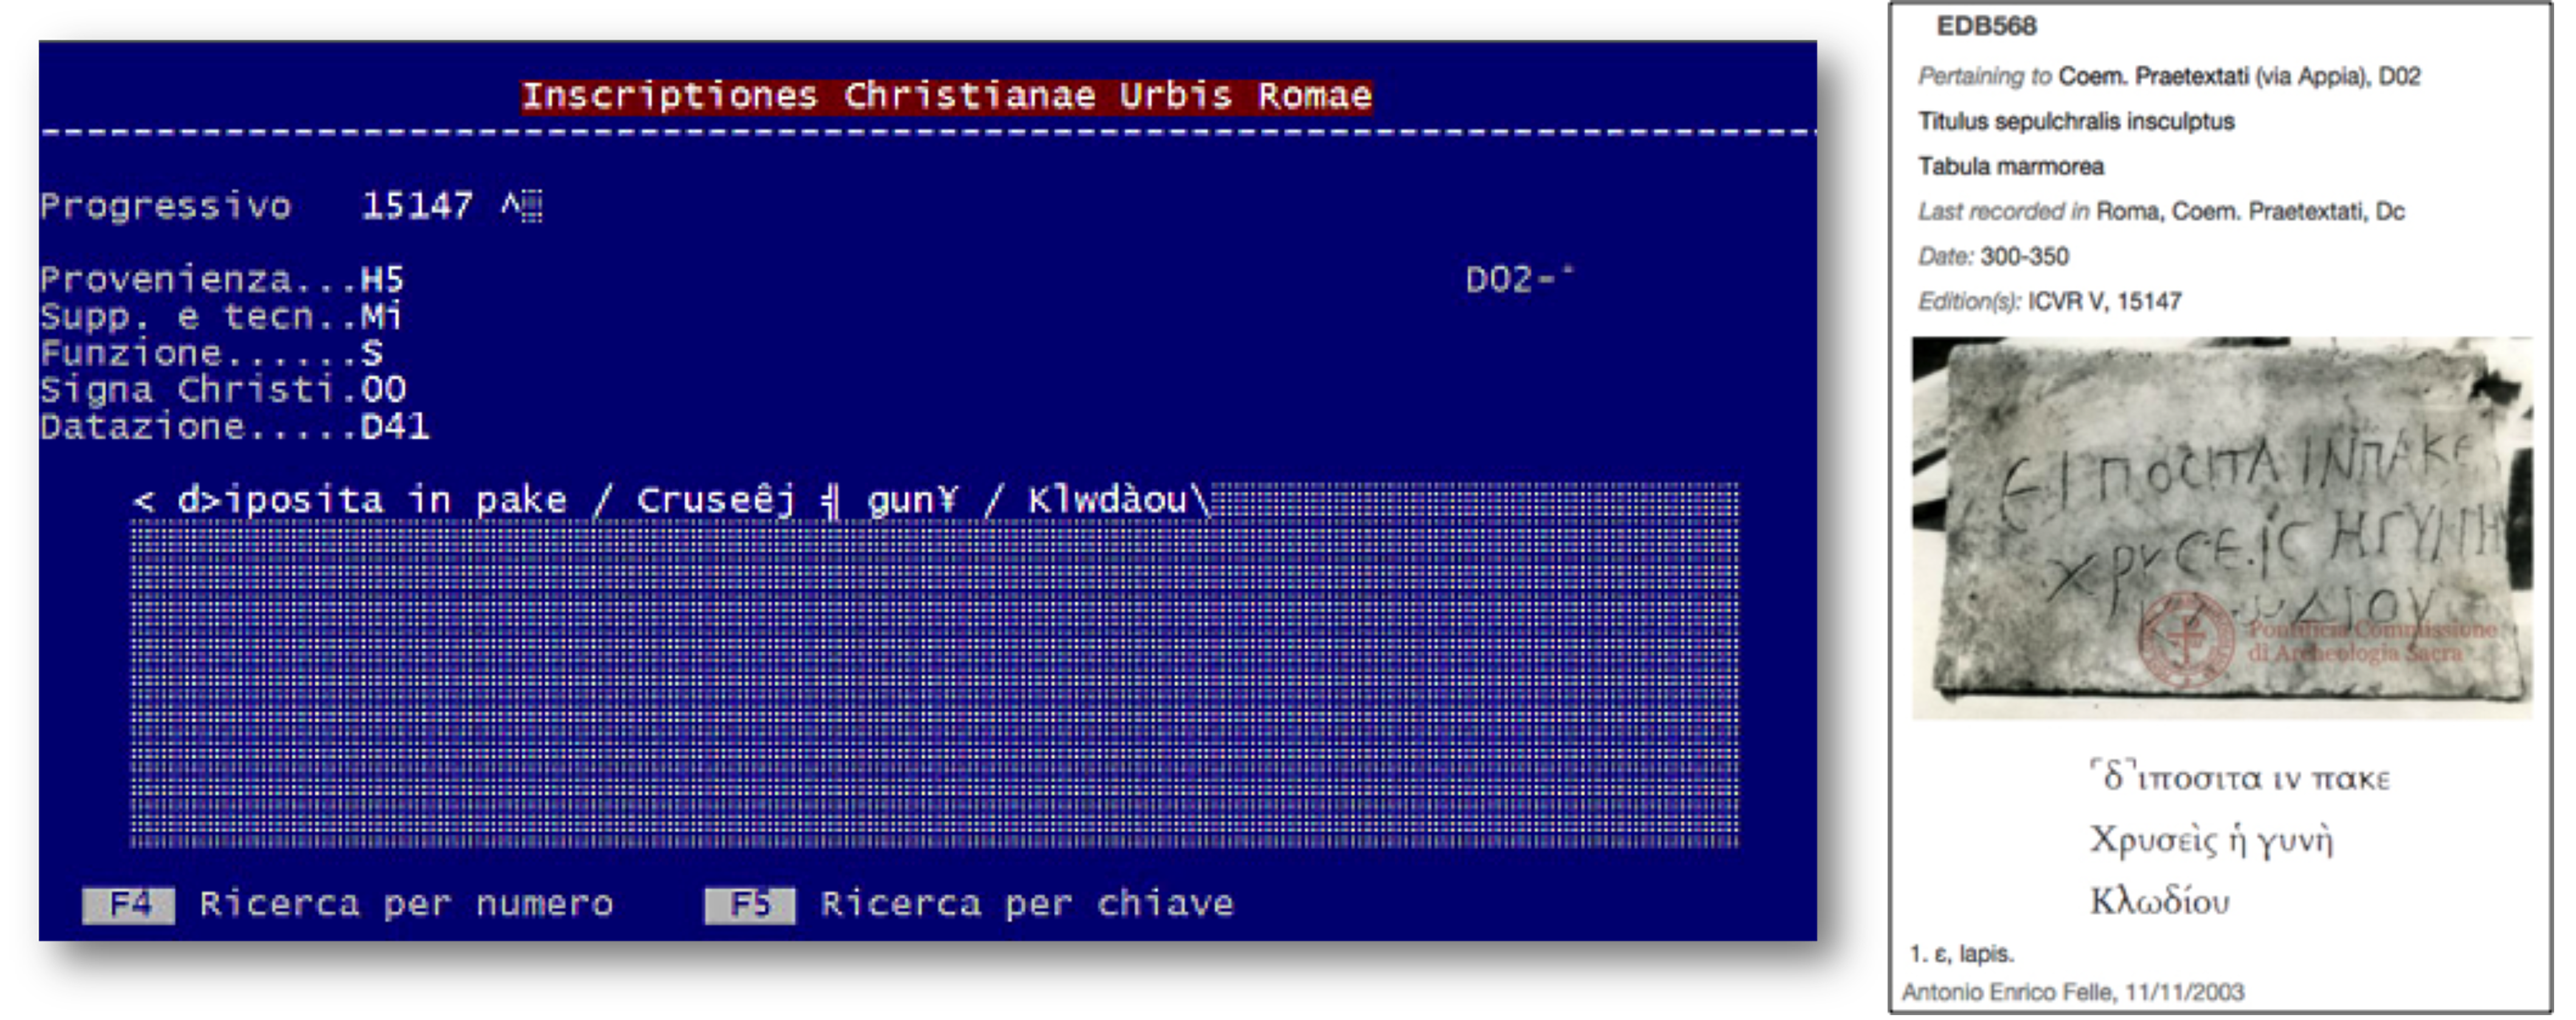
\includegraphics[width=\columnwidth]{Fig1NEW.png} 
\caption{The record of a bilingual inscription (ICVR V, 15147) as it appeared in data processing program ICVR in MS-DOS
in 1988 and as it appears now in EDB, with the acronyms expanded, the image and the text displayed in Greek characters.}
\label{fig:1}
\end{figure}




In addition to the text, the data processing program recorded for each inscription\footnote{ The program didn’t allow
the use of Greek fonts; in order to add texts in the Greek alphabet it was necessary to type Latin equivalent letters
in the MS Word \emph{Symbol} font, as you can see in Fig.~\ref{fig:1}}: bibliographic data (Progressivo = ICVR Number), origin
(Provenienza), type of support and technique of execution (Supp. e tecn.), function (Funzione), the presence or
absence of Christograms (\emph{Signa Christi}), and dating (Datazione). All this information was expressed by alphanumeric
codes of few characters, according to a limitation imposed by the program (Fig.~\ref{fig:1}).
%
%\begin{figure}[hbp]
%\centering
% \includegraphics[scale=0.4]{Fig.2.png} 
%\caption{The inscription ICVR V, 15147 as it appears now in EDB, with the acronyms expanded, the image and the text
%displayed in Greek characters.}
%\label{fig:2}
%\end{figure}
%



Adding metadata to the text, even if in the minimalistic form of alphanumeric codes, accomplished the goal of describing
the epigraphic object in its widest sense as an inscribed artifact. This feature, in particular relating to
geographical information, was even more meaningful according to the characteristics of a large part of the inscriptions
recorded in EDB. In fact, the original pertinence to a monument/container (catacomb) or to a particular area of it,
allows, with reasonable certainty, to determine the patronage by a member of the Christian community and moreover to
determine the chronology, even without specific references inside the text\footnote{\citet{carletti_inscriptiones_1994}; \citet[viii-ix]{felle_introduzione_1997}.}. Likewise reporting the presence of Christological monograms allows us to identify them as explicit symbols
of Christian faith and as chronological indicators\footnote{ The monogram consisting of the first two letters of the
name \begin{otherlanguage*}{greek}Χριστός\end{otherlanguage*} can be considered the archetype of these signs. They first appear in inscriptions at the
beginning of the fourth century.}. 

In the early 2000s, the ICVR database, containing more than 20,000 records, became part of the EAGLE federation of
databases (Electronic Archive of Greek and Latin Epigraphy), under the patronage of the Association Internationale
d’Épigraphie Grecque et Latine (AIEGL), as EDB (Epigraphic Database Bari) and extended its competencies to the
epigraphic documentation of Christian patronage of the city of Rome, published after the volumes of ICVR (Fig.~\ref{fig:3}). 

\begin{figure}[hbp]
\centering
 \includegraphics[width=\columnwidth]{EAGLE2016Roccoengrev-img003.png} 
\caption{The EDB homepage in 2004 and 2009.}
\label{fig:3}
\end{figure}



As a member of the federation, the database became available online through its own website and finally, thanks to the
EAGLE Europeana project, through a common portal.

Obviously this step has resulted in a series of changes and adjustments that led from the original basic structure of
the database to the present one. 

\section{The EDB structure}


The current structure of EDB consists of a relational database, based on the open-source program My-SQL, with a complex
scheme drafted according to the most recent advances in epigraphic methodology: reestablishing historical and material
value of the object, identifying each epigraph as a complex and polysemic product consisting partially but not only of
text (Fig.~\ref{fig:4}).



\begin{figure}[hbp]
\centering
 \includegraphics[width=\columnwidth]{EAGLE2016Roccoengrev-img004.png} 
\caption{The EDB database schema.}
\label{fig:4}
\end{figure}




\subsection{Bibliographic data}


As in the past version, the first pieces of information recorded for each epigraphic document are bibliographic data.

Besides data related to the ICVR publication - volume and edition number of the inscription - now EDB is able to record
other bibliographic references as well as concordances with other Corpora (CIL, IG, IGUR, IGC) (Fig.~\ref{fig:3b}). 

\newpage
\begin{figure}[!hbp]
\centering
 \includegraphics[width=\columnwidth]{Fig4.png}
\caption{Bibliographic data fields.}
\label{fig:3b}
\end{figure}


The whole bibliography is structured in metadata and is available both on the EDB website, and on the EAGLE BPN group of
Zotero\footnote{ \url{www.zotero.org/groups/eagleepigraphicbibliography/items }}, a tool for managing bibliographic data that
makes it easy to export entries and to cite them. An additional field allows the user to record references and links to
other online databases. 

It's even possible to define the relationship between the epigraph and the cited bibliography (printed or digital):
\emph{identity}, when it is an edition; \emph{integration}, if it's the edition of another fragment of the same inscription;
\emph{opistographic}, if it's the edition of the inscription on the back side; reuse, if it's the edition of another
inscription on the same support; \emph{comment}, if it's a study on a related topic.




\subsection{Geographic data}


One key element of differentiation of EDB from other similar projects is the structuring of the topographic data. 

This is due to the fact that the inscriptions of interest of EDB pertain only to the city of Rome, an area far more
limited than the large geographic ones managed by other epigraphic databases, but also and above all considering that,
as has been said previously, a large number of inscriptions of the Christians of Rome are still preserved in the place
for which they were created, sealing a tomb of an underground cemetery. Moreover, even if a given inscription isn't
still in its place on the grave, it is often still attributable to a specific area of the funerary complex.

Consequently in EDB, geographic indications require a more detailed articulation than in other databases, in which the
maximum level of definition is just the city of provenance, often lacking detailed information about the inscription’s
discovery.

Data on the \emph{original context} are therefore organized hierarchically in three related fields containing controlled lists (Fig.~\ref{fig:5}). 
After selecting the area of the suburb identified by the name of the consular road - or by the number of the Augustan
\emph{regio} for urban inscriptions - it's possible to select the monument from a list: a catacomb or part of it, if it is a
large and multi-layered one; a church; a public building or an urban area. The third field allows access to a further
associated list where the position of the epigraph inside the monument can be selected. For the catacombs in
particular, it’s possible to use these fields to annotate the gallery or the cubicle, named with the alphanumeric code
used in the maps published in ICVR.

\begin{figure}[hbp]
\centering
 \includegraphics[width=\columnwidth]{EAGLE2016Roccoengrev-img005.jpg} 
\caption{Original context input fields.}
\label{fig:5}
\end{figure}





Is worth noting that this set of associated fields refers to the original position of the inscriptions and not to the
place where they have been found, unless the two data coincide, that is in the case of inscriptions \emph{in situ} or \emph{suo loco
adplicitae}, in accordance with the definitions of the ICVR.

To complete information on spatial data, all cemeterial contexts have been georeferenced, so that clicking on their name
opens a new window in \emph{Google Map} that shows the modern entrance to the cemetery, with the address and its coordinates. 

As a case of study, for the inscriptions \emph{in situ} pertaining to the Domitilla catacomb (Via Ardeatina) - the only
cemeterial complex with a georeferenced plan of almost its entire extension\footnote{\emph{START-Projekt: Die
Domitilla-Katakombe in Rome (Institut für Kulturgeschichte der Antike - Österreichische Akademie der Wissenschaften)}.
\citet{orlandi_case_2014}.} - clicking on the alphanumeric code\footnote{ The codes are made up of a majuscule letter
relating to a region of the catacomb \ and by another element, digit or minuscule letter, relating to a precise
internal position, respectively a gallery or a \emph{cubiculum}. } associated to the precise position of the inscriptions,
gallery or \emph{cubiculum} (F04, in Fig.~\ref{fig:6}), opens the plan of the specific area (\emph{regio}) in which the inscription is found.
In every plan, the inscriptions preserved \emph{in situ} are placed and marked by ICVR and EDB number (Fig.~\ref{fig:6})\footnote{The
plans are available on START-Projektwebsite: \url{www.oeaw.ac.at/antike/index.php\&id=431}, clicking on EDB number opens a
window with the EDB record. }.

 \begin{figure}[!hbp]
\centering
 \includegraphics[width=\columnwidth]{EAGLE2016Roccoengrev-img006.png} 
\caption{The original context maps.}
\label{fig:6}
\end{figure}


Even the geographic data relating to the place of conservation of the inscriptions are managed with a similar structure.
Since not a few inscriptions, produced in Rome have been taken away and carried to other places in Italy or abroad, the
information have been organized in three related fields reporting respectively the list of the cities, the list of
associated structures, such as museums, churches or catacombs; and the specific positions in the context where the
object is actually preserved (Fig.~\ref{fig:7}).




\begin{figure}[hbp]
\centering
 \includegraphics[width=\columnwidth]{Fig7.png}
\caption{Conservation input fields.}
\label{fig:7}
\end{figure}




Adopting the best practice suggested by the EAGLE consortium, georeferencing is guaranteed even for the Conservation
data, linking every City/Town to GeoNames site\footnote{ \url{www.geonames.org}}, which allows the user to pinpoint the
location and to avoid ambiguity between homonyms. A link to the Trismegistos Collection\footnote{
\url{www.trismegistos.org}}, a database of papyrological and epigraphic collections, if available, also helps to identify
uniquely the place of conservation, as well as to obtain additional information, included the geographic
positioning (Fig.~\ref{fig:8new}).\footnote{\url{http://www.eagle-network.eu/wp-content/uploads/2013/06/EAGLE\_D2.2.2\_Content-harmonisation-guidelines-including-GIS-and-terminologies-Second-Release.pdf}}

\newpage
\begin{figure}[!hbp]
\centering
 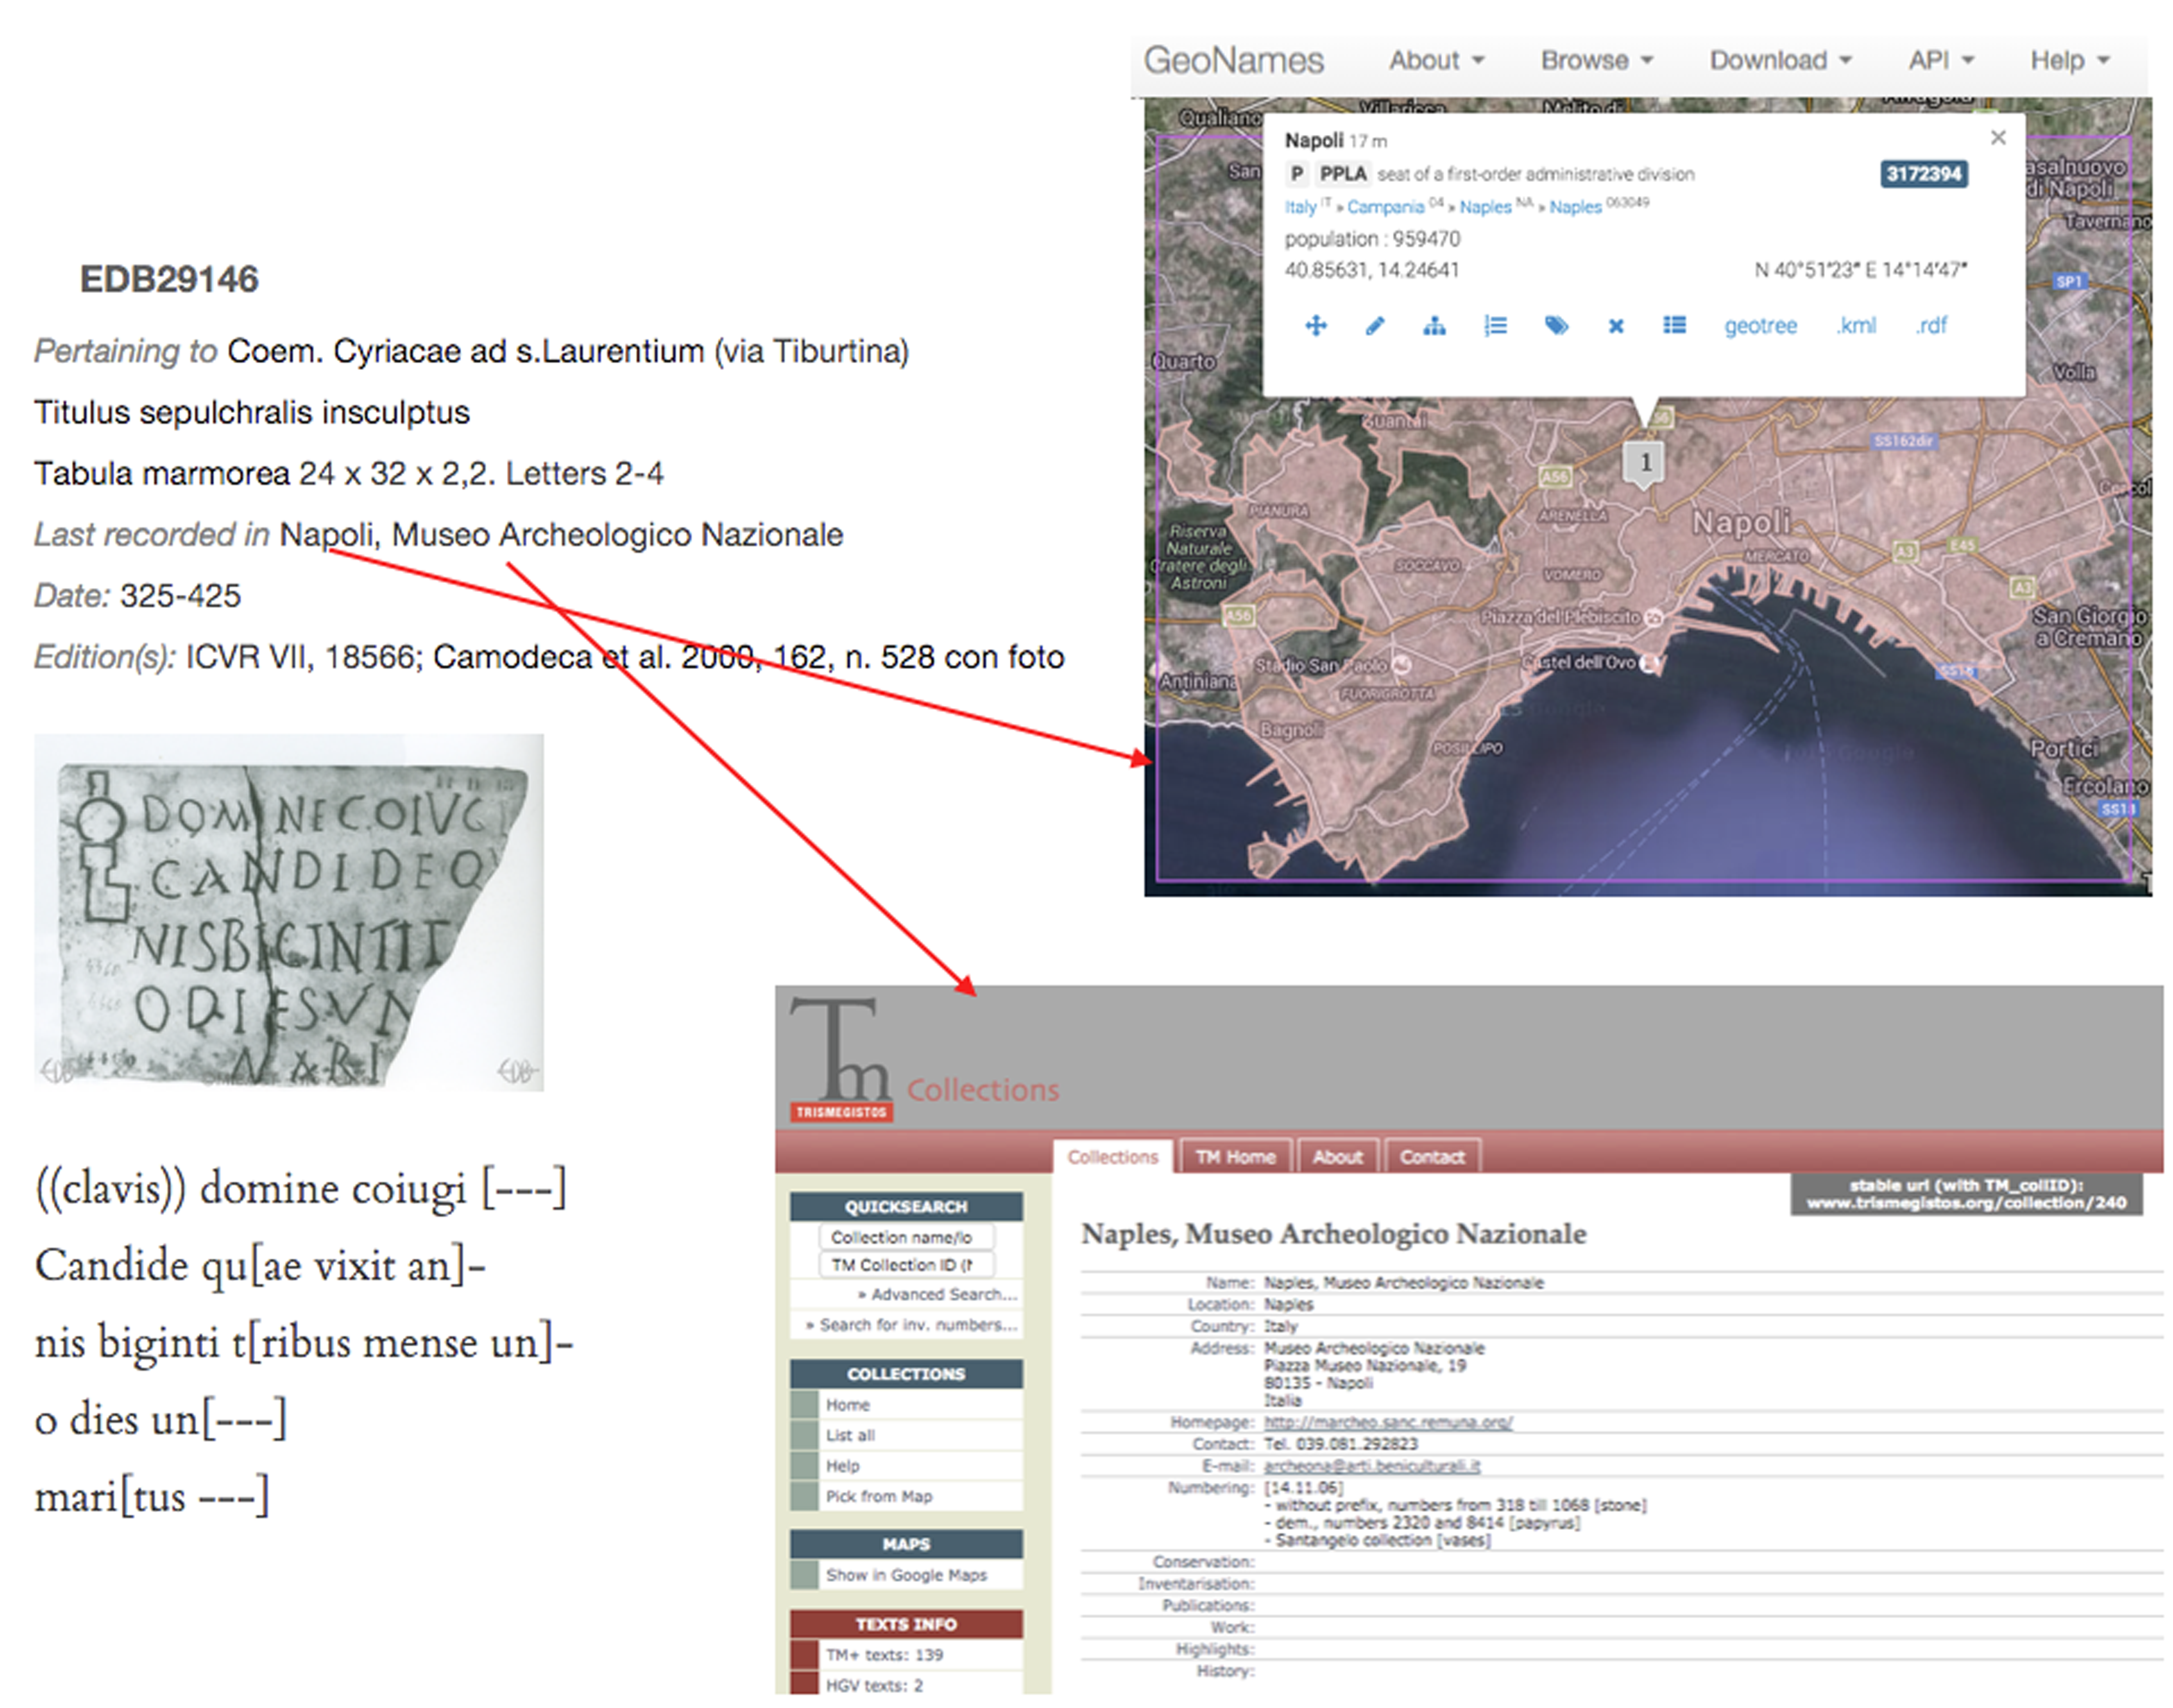
\includegraphics[width=\columnwidth]{Fig8.png}
\caption{Conservation maps and links.}
\label{fig:8new}
\end{figure}



\subsection{The description of the epigraphic object }


The nature of the inscription as material objects carrying textual information is represented by a series of attributes,
responding to the questions “What?” and “How?”: type of support and measures, technique of execution, height of letters
and paleographical features, and cases of reuse.

A survey of terminologies intended for description of epigraphic objects in the ICVR volumes has been carried out and
has generated lists of controlled terms for some of the fields (Fig.~\ref{fig:8}). \ \emph{Type of support}, \emph{Executing technique} and
\emph{Function} vocabularies are aimed at classifying the specific and peculiar materials, methods and functions of the
inscriptions encoded in EDB, as the traditional epigraphic taxonomies do not totally adhere to their features.

\begin{figure}[!hbp]
\centering
 \includegraphics[width=\columnwidth]{EAGLE2016Roccoengrev-img008.png}
\caption{Controlled vocabularies for Type of support, Executing technique and Function fields.}
\label{fig:8}
\end{figure}



The controlled lists have been integrated in the vocabularies of the EAGLE community\footnote{
\url{http://www.eagle-network.eu/resources/vocabularies/}.}, wich align, harmonize, create relations and translate into
various languages the terms used by the various partners, and returns them in a format that allows the user to get a
stable and unique identifier for each term, accessible and reusable by other users (Fig.~\ref{fig:9}).

\begin{figure}[!hbp]
\centering
 \includegraphics[width=\columnwidth]{EAGLE2016Roccoengrev-img009.png}
\caption{The integration with EAGLE Vocabularies, that can be opened clicking on the highlighted terms.}
\label{fig:9}
\end{figure}


\newpage

\subsection{The text}


The nature of the inscription as a sequence of characters carried by a physical object is represented by a series of
fields related to various features of texts: language and alphabet (Latin, Greek and the multiform combination of
coexistence between them), and metrical structure.

The proper text of the inscription is stored in an apposite field, following the Krummrey - Panciera
conventions\footnote{\citet{krummrey_criteri_1980}; \citet{Panciera1991}.}, with some adjustments to make it possible to describe
specific and peculiar issues of the inscriptions encoded in EDB. In particular the so-called
``aberrant'' forms are not ``normalized'' to the
``standard'' model, if they are recognized as grapho-phonetic outcomes of linguistic
modifications of Latin and Greek. 

While the fidelity to what is written on the stone - or other type of support - respects and takes into due account the
evolution of Greek and Latin languages, it compromises the comprehension of the text and greatly complicates the
text-based search of terms. A standard query system, in fact, is not able to match a query with all the inscriptions
containing different spellings of a word. To resolve this issue each inscription is stored in its original form and in
a ``lemmatized'' form, where each term is actually replaced with its corresponding lemma, possibly by taking into account
its inflexed forms\footnote{ On the contrary, if the compiler recognizes aberrant forms as outcomes of misstatements
and material mistakes of the stonecutters, he transcribes them with the appropriate corrections, following the Krummrey
- Panciera conventions. \citet{felle_perspectives_2014} e \citet{orlandi_improving_2014}.}.

In EDB, as in every epigraphic database, the transcription of the text provides a real pre-edition, with systematic
expansion of abbreviations, hypothesis of integration, and, if possible, an update version of the text, according to
recent publications. It includes, moreover, the description of non-alphabetic signs - in double round brackets - such
as figurative elements (fishes, birds, anchors, etc.) and Christological monograms. Other fields record onomastic
notes, \emph{critical apparatus} and textual comments (Fig.~\ref{fig:10}). 

A series of fields responding to the questions “When?” allows to insert a specific date, if recorded in the text, a
specific time span (such as the duration of the reign of a Bishop of Rome or of an emperor), or a generic interval.

\newpage

\begin{figure}[!hbp]
\centering
 \includegraphics[width=\columnwidth]{EAGLE2016Roccoengrev-img010.png}
\caption{Text fields in the submission mask.}
\label{fig:10}
\end{figure}




\subsection{The images}


Another meaningful improvement of EDB 2.0 is represented by the inclusion of visual representation of inscriptions. It’s
evident how images dramatically enhance analysis of epigraphic materials, showing them in their manifold aspects:
reference with the context, form and quality of the support, graphic forms, peculiarities of technique, layout and
relationship between the text and any figurative or decorative elements\footnote{\citet{panciera_questioni_2006}.}.

In the frame of the collaborations with Europeana, the largest online collection of digitized items, EDB has been
encouraged to enlarge the image repository, based on a cooperation agreement established between the EAGLE consortium
and the Ministry of Culture (MIBACT) and the Pontifical Commission for Sacred Archaeology (PCAS). A new uploading
process allowed tripling photos, squeezes and casts to be published online in low resolution and with a visible digital
watermark, respecting the restrictive Italian rules. A large portion of the digital images stored in the EDB repository
have been taken by collaborators during past years, and others have been scanned from publications, while a large
number come from the Photographic Archive of PCAS\footnote{ \url{www.archeologiasacra.net}}.




\section{Users, interface, search engine}





The system manages three kinds of users: editors, compilers and generic, anonymous ones.

The latter of these can navigate in the descriptive section of the website (About EDB, People) and in the list of cited
Publications. They also have access to the entire database using two research masks: a \emph{Quick search} allows the user to
search in only one of the following fields: identifier EDB, bibliographic data and text; an \emph{Advanced Search} provides
the opportunity to explore the database through multiple search criteria variously combined (Fig.~\ref{fig:11}).



\begin{figure}[!hbp]
\centering
 \includegraphics[width=\columnwidth]{EAGLE2016Roccoengrev-img011.png}
\caption{Quick and Advanced Search masks.}
\label{fig:11}
\end{figure}
 


Like today's web search engines, EDB provides an advanced text search in Latin and Greek - an integrated tool
facilitates writing in the Greek alphabet\footnote{ \emph{Greek Inputter 2}, developed by J. Naughton, allows the user to
write in Greek using his/her usual keyboard and to easily type various Greek diacritical marks
(\url{http://babel.mml.ox.ac.uk/ naughton / polytonic-greek-inputter.html}).} - allowing users to obtain different results
according to a default syntax, in the case of a search either for a single word or for a set of terms, in sequence or
not. Additionally, it's possible to choose whether or not to consider epigraphic diacritical marks, Greek accents and
spirits, and capitals. The textual search can be combined with other metadata related to bibliographic, geographic and
material data, or to function, reuse, language and date, expressed in a single year or in defined intervals. 

This wide range of possibilities has been designed to reach users with different needs: the occasional user looking for
a particular inscription could just type one or more words that he is able to read and decipher, and the specialist
user, who can access detailed information about a single epigraph or use the advanced search to query the database
about groups of documents with common characteristics. 

The search results are listed in a table showing the EDB identifier, bibliographic data, place of origin and place of
conservation, text of the inscription and a link to the full record.




\section{Conclusions}


This paper briefly describes the growth of Epigraphic Database Bari in nearly the last thirty years, from the first
experimental and minimalistic version, intended just for the use of a small group of researchers of Bari University, to
the present one, open to a large public of curious curious individuals, students and, of courses, specialists.

The involvement in the EAGLE – Europeana project, network of Ancient Greek and Latin Epigraphy, has had a significantly
positive impact on the development of the database of inscriptions by Christians from Rome. 

In fact, although EDB, like other partner databases, has maintained its character, dictated by its own history and,
mostly, by the characteristics of its documentary base, it has taken advantage of the solutions adopted to integrate
different archives and purpose-built best practices. 

Among the improvements, it’s worth mentioning

\begin{enumerate}
\item The inclusion of EDB bibliography, structured in metadata, in the Zotero Group, where it has been merged with those
of other content providers and has been made directly and publicly available in the most reusable way, giving more
exposition of the bibliographic database; allowing the integration and enrichment with other databases; allowing easy
export of data in multiple formats (bibtex, bookmarks, mods, rdf, xml, etc).

\item Following EAGLE best practice suggestions, data about modern places have been enriched with links to reference
resources, such as GeoNames and the Trismegistos Collection\footnote{
\url{http://www.eagle-network.eu/wp-content/uploads/2013/06/EAGLE\_D2.2.2\_Content-harmonisation-guidelines-including-GIS-and-terminologies-Second-Release.pdf}},
extending the use of stable and unique identifier accessible and reusable by other users (URI).

\item With the same aim, the controlled lists of \emph{Type of support}, \emph{Executing technique} and \emph{Function} have been integrated in
the corresponding vocabularies of the EAGLE community. Among other benefits, such as alignment and relations between
databases, clicking on specific terms opens an EAGLE vocabulary window with a translation into various languages. This
feature is particularly useful in the case of EDB which, following ICVR, uses Latin for definitions, without modern
language translations.

\item Encouraged by the collaborations with Europeana, EDB has tripled the number of images stored in its repository,
including inedited images taken by collaborators over the years. 
\end{enumerate}


On the other hand, EDB, being inside Eagle since its origin, has been a bridgehead for the non standard epigraphies,
proposing issues to the Eagle community and pushing to make the data model more flexible. For example, EDB asked to add
more than one technique of execution for a single support and to add more than one language and / or alphabet for the
same inscription, change that is indispensable to describe bilingual and/or bigraphic texts. 

Other solutions adopted in EDB could be, in the future, suitable for other projects, such as the hierarchic and
multi-step organization of topographic data, which could be applied to closed contexts of any age (houses, columbaria,
and so on) as well as the treatment of aberrant forms and the lemmatization process, which could be applied to any non
standard language. 

\nocite{felle_fenomeni_2007}
\nocite{felle_esperienze_2012}
\nocite{jory_problems_1975}
\nocite{Rocco2015a}

\section*{Acknowledgement}
The author would like to acknowledge the support of the European Commission through the
EAGLE project - Europeana network of Ancient Greek and Latin Epigraphy (Grant no: 325122). Moreover, the author thanks
Carlo Carletti, Antonio E. Felle, Filippo A. Piazzolla, Marida Pierno, and Gianvito Pio who daily use EDB and manage
the input of inscriptions and metadata, and the entire EAGLE community, which creates a space of real networking,
debate and the sharing ideas and data.

\section*{Corpora}
\begin{description}
\item[CIL] = \emph{Corpus Inscriptionum Latinarum}, \ Berolini 1863 ss.
\item[CIG] = \emph{Corpus Inscriptionum Grecarum}, I-IV, Berolini 1828-1877
\item[IC] = \emph{Inscriptiones christiane urbis Romae septimo saeculo antiquiores}, I-II, G.B. de Rossi (a c.), Romae 1857-1861; \emph{Supplementum}, G. Gatti (a c.), Romae 1915. 
\item[IG] = \emph{Inscriptiones Graecae}, Berolini 1873 ss.
\item[ICVR] = \emph{Inscriptiones christianae urbis Romae septimo saeculo antiquiores. Nova series}, I-X, A. Silvagni, A. Ferrua, D. Mazzoleni, C. Carletti (a c.), Romae - In Civitate Vaticana 1922 ss.
\item[IGVR] = \emph{Inscriptiones grecae urbis Romae}, I-IV, L. Moretti (a c.), Roma 1968-1990. 

\end{description}

\bibliographystyle{sapauth-eng}
\bibliography{../../EAGLE}

\end{document}
